\cleardoublepage
\chapter{Installing and configuring Scrappy}
\label{apdx:installscrappy}

This tutorial goes through the process of installing and configuring Scrappy to be able crawl services for the OMELETTE project.
Scrappy's code is available at https://github.com/gsi-upm/scrappy However, in order to use it with OMR, we have introduced some modifications. The new code can be found in the branch "omr".


\section{Installation}
\subsection{Requirements}
\begin{itemize}
	\item Graphviz
	\item Raptor library: raptor-utils
	\item Ruby 1.8
	\item Ruby Gems
	\item Sesame 2.0\footnote{http://www.openrdf.org/doc/sesame2/users/ch06.html} If the rdf is stored in sesame server.
	\item The gems listed below should be installed. In linux, this can be done, for example 'sudo gem install nokogiri'.
	\begin{itemize}
		\item nokogiri 1.5.4
		\item lightrdf 0.4.1
		\item i18n 0.6.0
		\item iconv 0.1
		\item multi\_json 1.3.6
		\item ntlm-http 0.1.1
		\item webrobots 0.0.13
		\item sinatra 1.3.2
		\item sinatra-flash 0.3.0
		\item eventmachine 0.12.10
		\item mechanize 2.5.1
		\item tilt 1.3.3
		\item haml
		\item rack 1.4.2
		\item rack-protection 1.2.0
		\item rack-flash 0.1.2
	\end{itemize}
\end{itemize}

\subsection{Installation steps}
\begin{itemize}
	\item Install ruby and rubygems
	\item Scrappy can be installed as a standard Ruby gem. However, some of the above gems may have extra dependencies. In particular, nokogiri requires several system libraries to be installed, and sinatra-flash may not be automatically installed, so you need to install then manually before installing scrappy:
	\begin{lstlisting}[style=consola, numbers=none]
		sudo apt-get install ruby-dev libxslt-dev libxml2-dev
		sudo gem install sinatra-flash
		sudo gem install scrappy
	\end{lstlisting}
	
	\item If you want to run scrappy with the OMR, you need to get the modified version from github, of both scrappy and lightrdf.
	
		\begin{lstlisting}[style=consola, numbers=none]
			git clone https://github.com/gsi-upm/scrappy.git
			git clone https://github.com/gsi-upm/lightrdf.git
			cd scrappy
			git checkout omr
			cd ../lightrdf
			git checkout omr
		\end{lstlisting}

	
\end{itemize}

This will create a folder named “scrappy”, (along with the new lightrdf folder). Inside it, in the “bin” subdirectory you can find the runnable for scrappy. Be careful to maintain the scrappy and lightrdf folder in the same directories, so scrappy can find the correct lightrdf to load.

\section{User manual}
\label{sec:scrappyusermanual}
Scrappy provides a set of interfaces to extract RDF from a web page. In order to see the available options, the user can execute 'scrappy –help' as follows.

\begin{lstlisting}[style=consola, numbers=none]
scrappy --help

Scrappy v0.4.10
Synopsis
Scrappy is a tool to scrape semantic data out of the unstructured web
Examples
This command retrieves a web page
scrappy -g http://www.example.com
Usage
scrappy [options]
For help use: scrappy -h
Options
-h, --help
Displays help message
-v, --version
Displays the version, then exits
-f, --format
Picks output format (json, ejson, rdf, ntriples, png)
-g, --get URL
Gets requested URL
-p, --post URL
Posts requested URL
-c, --concurrence VALUE Sets number of concurrent connections for crawling (default is
10)
-l, --levels VALUE
Sets recursion levels for resource crawling (default is infinite
crawling)
-d, --delay VALUE
Sets delay (in ms) between requests (default is 0)
-D, --dump
Dumps RDF data to disk
-u, --debug [KEYWORD] Shows debugging traces. Use optional keyword to filter
selectors' output
-o, --observe URLs
Observes the specified URLs storing their data into the repository
-s, --server [ROOT]
Runs web server (optionally specify server's root url)
-a, --admin [ROOT]
Runs admin web server (optionally specify server's root url)
-P, --port PORT
Selects port number (default is 3434)
-t, --time TIME
Returns repository data from the last given minutes
\end{lstlisting}

Scrappy provides several interfaces: command line interface, web admin interface, web
service interface and Ruby interface.

\subsection{Command line interface}

The command line interface can be used in a command shell window as shown in Figure 2.
For example, the web example.com can be scraped with the following command.

\begin{lstlisting}[style=consola, numbers=none]
	scrappy -g example.com
\end{lstlisting}
For example, the output from google.com would look like the following window. Be advised:
most of the times the RDF data will not fit in a single window, so its recommended to pipe it to
another command or a text file.

\begin{figure}[h]
	\centering
	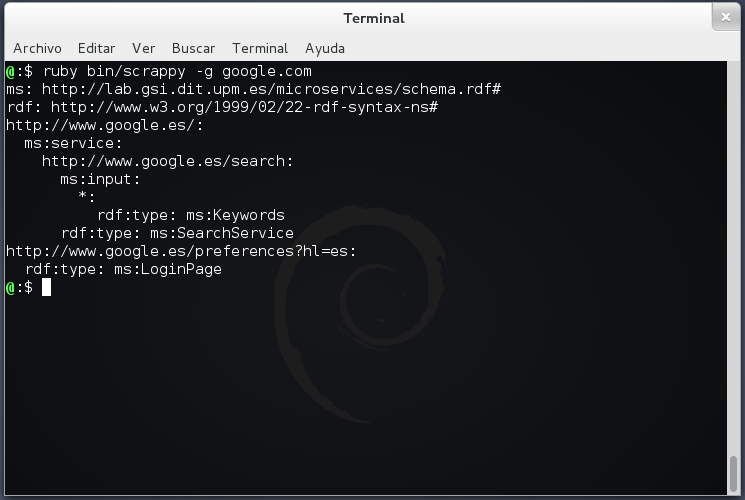
\includegraphics[width=400pt]{graphics/scrappy-cmd.png}
	\caption{Scrappy command line interface}
	\label{fig:scrappycmd}
\end{figure}

\subsection{Web admin interface}
The web admin interface can be used in a regular web browser, to either scrape a site or
browse the different resources, such as the extractors. To launch it, you need to open a
command line, and execute the following command:

\begin{lstlisting}[style=consola, numbers=none]
scrappy -a
Launching Scrappy Web Admin (browse http://localhost:3434)...
== Sinatra/1.1.3 has taken the stage on 3434 for production with backup from Thin
\end{lstlisting}

Once scrappy has been launched, user can access the admin interface (Figure \ref{fig:scrappyweb}). In order to
scrape a web site, it is only required to introduce the URI and select the desired output (RDF,
JSON, YARF or PNG).

\begin{figure}[h]
	\centering
	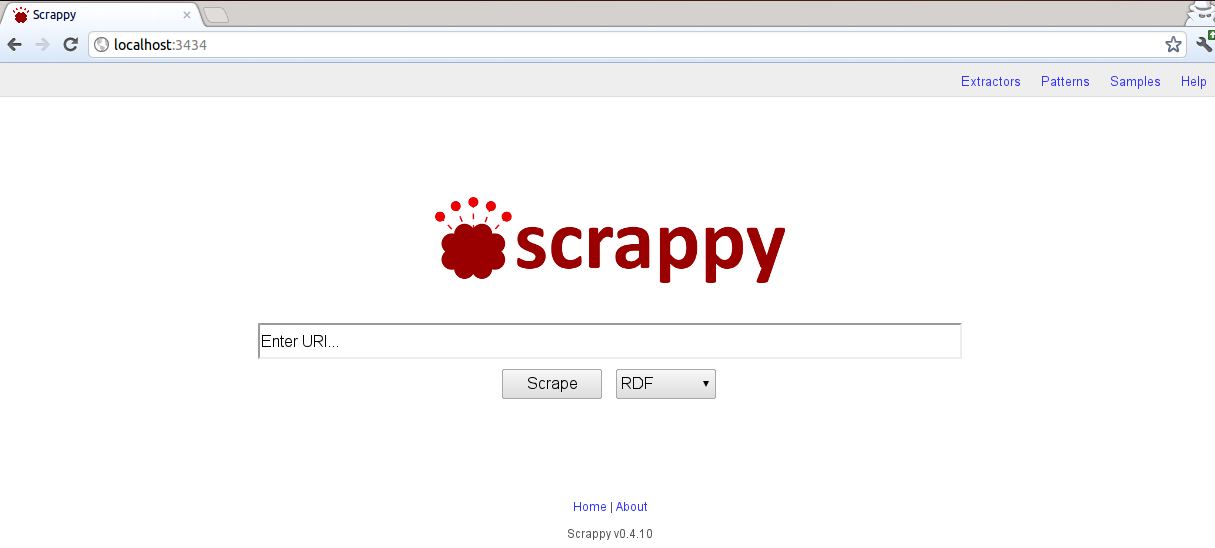
\includegraphics[width=400pt]{graphics/scrappy-web.png}
	\caption{Web admin interface of Scrappy}
	\label{fig:scrappyweb}
\end{figure}

This interface also allows managing the extractors from each page (extractor tab, Figure \ref{fig:scrappyextractors}),
define visual patterns for improving the extraction (patterns) and train the extractors (samples
tab). These last two tabs are still experimental facilities, so and end user would not need to
use them.

\begin{figure}[h]
	\centering
	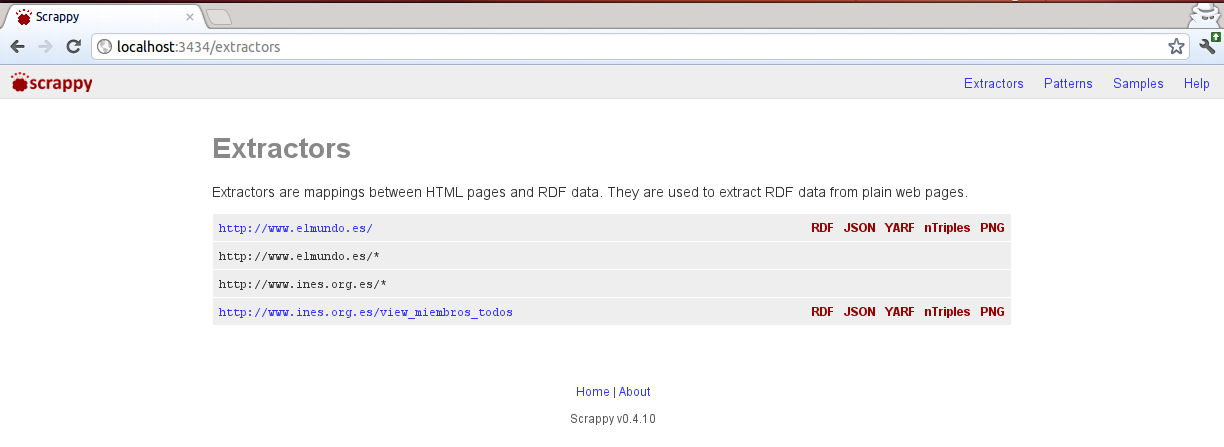
\includegraphics[width=400pt]{graphics/scrappy-extractors-interface.png}
	\caption{Extractors Admin Interface}
	\label{fig:scrappyextractors}
\end{figure}

\subsection{Web service interface}
The web service interface provides a web service interface that mimics the admin web
interface but for read-only operations.

\begin{lstlisting}[style=consola, numbers=none]
scrappy -s
Launching Scrappy Web Server...
== Sinatra/1.1.3 has taken the stage on 3434 for production with backup from Thin
\end{lstlisting}

This service does not provide a front page, so you need to make a GET petition to a specific
url, following this syntax: http://[scrappyhost:port]/[format]/[url]. For example, to get rdf data
out of example.com, launching scrappy in localhost with the default port, it would be:
http://localhost:3434/rdf/example.com.

\subsection{Ruby interface}
Scrappy can be used in a Ruby program by requiring the gem.

\begin{lstlisting}[style=consola]
require 'rubygems'
require 'scrappy'
# Parse a knowledge base
kb = RDF::Parser.parse :yarf,
open("https://raw.github.com/gsi-upm/scrappy/omr/extractors/programmableweb.yarf").re
ad
# Set kb as default knowledge base
Scrappy::Agent::Options.kb = kb
# Create an agent
agent = Scrappy::Agent.new
# Get RDF output
output = agent.request :method=>:get, :uri=>'http://www.programmableweb.com'
# Output all titles from the web page
titles = output.find([], Node('dc:title'), nil)
titles.each { |title| puts title }
\end{lstlisting}

For example, to extract the data from http://www.programmableweb.com, you will need:

\begin{lstlisting}[style=consola]
require 'rubygems'
require 'scrappy'
# Parse a knowledge base
kb = RDF::Parser.parse :yarf,
open("HOME_DIR/.scrappy/extractors/programmableweb.yarf").read
# Set kb as default knowledge base
Scrappy::Agent::Options.kb = kb
# Create an agent
agent = Scrappy::Agent.new
# Get RDF output
output = agent.request :method=>:get, :uri=>'http://www.programmableweb.com'
# This will return a graph object. To get the ntriples
# ntriples
ntriples = output.serialize :ntriples
# rdf
rdf = output.serialize :rdf
\end{lstlisting}

\subsection{Integration with Sesame}
While using OMR, several modifications have been introduced into scrappy, in order
to user both Sesame and OMR. The new configuration file includes the options to connect to
both platforms:

\newpage
\begin{lstlisting}[style=consola]
# The host were omr is. Do not add the trailing '/'
omr_host: https://vsr-web.informatik.tu-chemnitz.de/
omr_complete: omr-write/components
omr_user: omr-user
omr_pass: omr-pass
omr_port: 443
# The time to consider the data in the repository valid, in minutes
time: 5
# The format to communicate with the repository
format: ntriples
# You can use any of the following formats:
# rdf, ntriples, turtle, n3, trix, trig
\end{lstlisting}

In general, it has the same values as a normal scrappy config file has, but, also, several
“omr” values:

\begin{itemize}
\item complete: how to complete the url for the sesame server.
\item omr\_host: The host where omr is installed
\item omr\_complete: how to complete the url for omr.
\item omr\_user: the user to connect with omr
\item omr\_pass: The password for the given user
\item omr\_port: The port for the connection. Since omr uses https, the default port is 443
\end{itemize}

\subsection{Extractors}

Extractors are based on the Scraping ontology and define mappings between HTML content
and RDF data. An example of extractor is shown in Listing \ref{lst:extractorExample}.


\begin{lstlisting}[style=mono,breaklines=true,label={lst:extractorExample}, caption=Extractor example for Yahoo! Pipes]
dc: http://purl.org/dc/elements/1.1/
owl: http://www.w3.org/2002/07/owl#
rdf: http://www.w3.org/1999/02/22-rdf-syntax-ns#
rdfs: http://www.w3.org/2000/01/rdf-schema#
sioc: http://rdfs.org/sioc/ns#
sc: http://lab.gsi.dit.upm.es/scraping.rdf#
vu: http://vulneranet.org/vulneranet.owl#
omelette: http://www.ict-omelette.eu/schema.rdf#
ctag: http://commontag.org/ns#
rosm: http://www.wsmo.org/ns/rosm/0.1#
hrests: http://www.wsmo.org/ns/hrests#

# Home page
*:
  rdf:type: sc:Fragment
  sc:selector:
    *:
      rdf:type: sc:UriSelector
      rdf:value: "http://pipes.yahoo.com/pipes/"
  sc:subfragment:
    *:
      rdf:type: sc:Fragment
      sc:type: sc:Index
      sc:selector:
        *:
          rdf:type: sc:CssSelector
          rdf:value: "a.navlink"
          sc:keyword: "browse"
      sc:identifier:
        *:
          rdf:type: sc:RootSelector
          sc:attribute: "href"

# Popular pipes page
*:
  rdf:type: sc:Fragment
  sc:selector:
    *:
      rdf:type: sc:UriSelector
      rdf:value: "http://pipes.yahoo.com/pipes/pipes.popular"
  sc:subfragment:
    *:
      rdf:type: sc:Fragment
      sc:type: sc:Page
      sc:selector:
        *:
          rdf:type: sc:CssSelector
          rdf:value: "#mTagstoptags a"
      sc:identifier:
        *:
          rdf:type: sc:NewUriSelector
          sc:prefix: "http://pipes.yahoo.com/pipes/search?r=tag:"
          sc:follow: "true"
          sc:downcase: "true"

# Any index page
*:
  rdf:type: sc:Fragment
  sc:selector:
    *:
      rdf:type: sc:UriSelector
      rdf:value:
        "http://pipes.yahoo.com/pipes/pipes.popular"
        "http://pipes.yahoo.com/pipes/search"
  sc:subfragment:
    *:
      rdf:type: sc:Fragment
      sc:type: omelette:Service
      sc:selector:
        *:
          rdf:type: sc:CssSelector
          rdf:value: "li.pipelistli"
      sc:identifier:
        *:
          rdf:type: sc:CssSelector
          rdf:value: "h3 a"
          sc:attribute: "href"
      sc:subfragment:
        *:
          rdf:type: sc:Fragment
          sc:relation: omelette:dataFormat
          sc:type: rdf:Literal
          sc:selector:
            *:
              rdf:type: sc:CssSelector
              rdf:value: "li.first"
              sc:keyword: "formats:"
              sc:selector:
                *:
                  rdf:type: sc:XPathSelector
                  rdf:value: "./../li[@class='tag']/a"
    *:
      rdf:type: sc:Fragment
      sc:type: sc:Page
      sc:selector:
        *:
          rdf:type: sc:CssSelector
          rdf:value: ".paginate a"
          sc:keyword: "next >"
      sc:identifier:
        *:
          rdf:type: sc:RootSelector
          sc:attribute: "href"

# Yahoo Pipe
*:
  rdf:type: sc:Fragment
  sc:type: omelette:Service
  sc:selector:
    *:
      rdf:type: sc:UriPatternSelector
      rdf:value: "http://pipes.yahoo.com/pipes/pipe.info?_id=*"
  sc:identifier:
    *:
      rdf:type: sc:BaseUriSelector
  sc:subfragment:
    *:
      rdf:type: sc:Fragment
      sc:relation: rdfs:label
      sc:type: rdf:Literal
      sc:selector:
        *:
          rdf:type: sc:CssSelector
          rdf:value: "h1.title"
    *:
      rdf:type: sc:Fragment
      sc:relation: dc:description
      sc:type: rdf:Literal
      sc:selector:
        *:
          rdf:type: sc:CssSelector
          rdf:value: ".bd .desc"

    *:
      rdf:type: sc:Fragment
      sc:relation: ctag:tagged
      sc:type: ctag:Tag
      sc:selector:
        *:
          rdf:type: sc:CssSelector
          rdf:value: "#mTagstoptags a"
      sc:identifier:
        *:
          rdf:type: sc:NewUriSelector
          sc:prefix: "http://www.ict-omelette.eu/omr/tags/"
          sc:downcase: "true"
      sc:subfragment:
        *:
          rdf:type: sc:Fragment
          sc:type: rdf:Literal
          sc:relation: rdfs:label
          sc:selector:
            *:
              rdf:type: sc:RootSelector

    *:
      rdf:type: sc:Fragment
      sc:relation: omelette:uses
      sc:selector:
        *:
          rdf:type: sc:CssSelector
          rdf:value: "#mSourcestoptags a"
      sc:identifier:
        *:
          rdf:type: sc:NewUriSelector
          sc:prefix: "http://"
          sc:downcase: "true"

    *:
      rdf:type: sc:Fragment
      sc:relation: omelette:uses
      sc:type: omelette:Service
      sc:selector:
        *:
          rdf:type: sc:CssSelector
          rdf:value: "#mModulestoptags a"
      sc:identifier:
        *:
          rdf:type: sc:NewUriSelector
          sc:prefix: "http://www.ict-omelette.eu/omr/operator/"
          sc:downcase: "true"
      sc:subfragment:
        *:
          rdf:type: sc:Fragment
          sc:type: rdf:Literal
          sc:relation: rdfs:label
          sc:selector:
            *:
              rdf:type: sc:RootSelector
    *:
      rdf:type: sc:Fragment
      sc:relation:
        omelette:endpoint
        dc:source
      sc:selector:
        *:
          rdf:type: sc:RootSelector
      sc:identifier:
        *:
          rdf:type: sc:BaseUriSelector

    *:
      rdf:type: sc:Fragment
      sc:relation: omelette:describedBy
      sc:type: rosm:Service
      sc:selector:
        *:
          rdf:type: sc:RootSelector
      sc:subfragment:
        *:
          rdf:type: sc:Fragment
          sc:relation: rosm:supportsOperation
          sc:type: rosm:Operation
          sc:selector:
            *:
              rdf:type: sc:RootSelector
          sc:subfragment:
            *:
              rdf:type: sc:Fragment
              sc:relation: hrests:hasAddress
              sc:selector:
                *:
                  rdf:type: sc:BaseUriSelector
              sc:identifier:
                *:
                  rdf:type: sc:NewUriSelector
                  sc:suffix: "&_render=rss"
            *:
              rdf:type: sc:Fragment
              sc:relation: rosm:requestURIParameter
              sc:selector:
                *:
                  rdf:type: sc:CssSelector
                  rdf:value: "#runform table input[@type!='submit']"
              sc:subfragment:
                *:
                  rdf:type: sc:Fragment
                  sc:relation: rdfs:label
                  sc:type: rdf:Literal
                  sc:selector:
                    *:
                      rdf:type: sc:RootSelector
                      sc:attribute: "name"
                *:
                  rdf:type: sc:Fragment
                  sc:relation: ctag:tagged
                  sc:selector:
                    *:
                      rdf:type: sc:RootSelector
                      sc:attribute: "type"
                  sc:subfragment:
                    *:
                      rdf:type: sc:Fragment
                      sc:type: rdf:Literal
                      sc:relation: rdfs:label
                      sc:selector:
                        *:
                          rdf:type: sc:RootSelector
                          sc:attribute: "type"

elector
              rdf:value: "a"
\end{lstlisting}

